\documentclass[12pt,a4paper]{article}% 文档格式
\usepackage{ctex}% 输出汉字
\usepackage{times}% 英文使用Times New Roman

% 数学公式
\usepackage{amsmath,amsfonts,amssymb}% 为公式输入创造条件的宏包
\usepackage{array}
\usepackage{bm} % 公式加粗
% \mathversion{bold}  % 设置数学字母、公式加黑加粗

% 图片
\usepackage{graphicx}% 图片插入宏包
\usepackage{subfigure}% 并排子图
\usepackage{float}% 浮动环境,用于调整图片位置
\usepackage[export]{adjustbox}% 防止过宽的图片

% 参考文献
\usepackage{bibentry}
\usepackage[square,sort,comma,numbers]{natbib}% 以上2个为参考文献宏包

% 两栏文档,一栏摘要及关键字宏包
\usepackage{abstract}
\renewcommand{\abstracttextfont}{\fangsong}% 摘要内容字体为仿宋
\renewcommand{\abstractname}{\textbf{摘\quad 要}}% 更改摘要二字的样式

% 字体颜色宏包
\usepackage{xcolor}
\newcommand{\red}[1]{\textcolor[rgb]{1.00,0.00,0.00}{#1}}
\newcommand{\blue}[1]{\textcolor[rgb]{0.00,0.00,1.00}{#1}}
\newcommand{\green}[1]{\textcolor[rgb]{0.00,1.00,0.00}{#1}}
\newcommand{\darkblue}[1]
{\textcolor[rgb]{0.00,0.00,0.50}{#1}}
\newcommand{\darkgreen}[1]
{\textcolor[rgb]{0.00,0.37,0.00}{#1}}
\newcommand{\darkred}[1]{\textcolor[rgb]{0.60,0.00,0.00}{#1}}
\newcommand{\brown}[1]{\textcolor[rgb]{0.50,0.30,0.00}{#1}}
\newcommand{\purple}[1]{\textcolor[rgb]{0.50,0.00,0.50}{#1}}% 为使用方便而编辑的新指令

\usepackage{url}% 超链接
\usepackage[hidelinks]{hyperref}   % 链接引用
\usepackage{multirow}
\usepackage{booktabs}
\usepackage{epstopdf}
\usepackage{epsfig}
\usepackage{longtable}% 长表格
\usepackage{supertabular}% 跨页表格
\usepackage{algorithm}
\usepackage{algorithmic}
\usepackage{changepage}% 换页
\usepackage{enumerate}% 短编号

\usepackage{enumitem}           %调整列举环境
% 列表设置
\setenumerate{fullwidth,itemindent=\parindent,listparindent=\parindent,itemsep=0ex,partopsep=0pt,parsep=0ex}
\setenumerate[2]{label=\alph*,leftmargin=1em}  %二级item设置
\setitemize{itemindent=38pt,leftmargin=0pt,itemsep=-0.4ex,listparindent=26pt,partopsep=0pt,parsep=0.5ex,topsep=-0.25ex}
\setdescription{itemindent=38pt,leftmargin=0pt,itemsep=-0.4ex,listparindent=26pt,partopsep=0pt,parsep=0.5ex,topsep=-0.25ex}

% 标题及标题格式
\usepackage{caption}
% \usepackage{subcaption}
\captionsetup[figure]{name=\selectfont \textbf{图}}% 设置图片编号头
\captionsetup[table]{name=\selectfont \textbf{表}}% 设置表格编号头
% 图的标题行间距设置
\setlength{\abovecaptionskip}{0.5em}
\setlength{\belowcaptionskip}{-0.8em}

% 缩进及页边距
\usepackage{indentfirst}% 中文首行缩进
\usepackage[left=2.50cm,right=2.50cm,top=2.80cm,bottom=2.50cm]{geometry}% 页边距设置
\renewcommand{\baselinestretch}{1.5}% 定义行间距(1.5)

% 插入代码
\usepackage{listings}
\usepackage{xcolor}
% 代码格式设置
\lstset{
 columns=fixed,
 numbers=left,                                        % 在左侧显示行号
 numberstyle=\footnotesize\color{gray},                       % 设定行号格式
 frame=single,                                        % 单线背景边框
 breaklines=true,                                     % 设定LaTeX对过长的代码行进行自动换行
 keywordstyle=\color[RGB]{40,40,255},                 % 设定关键字颜色
 numberstyle=\footnotesize\color{darkgray},
 commentstyle=\it\color[RGB]{0,96,96},                % 设置代码注释的格式
 stringstyle=\rmfamily\slshape\color[RGB]{128,0,0},   % 设置字符串格式
 showstringspaces=true,                              % 不显示字符串中的空格
 language=Matlab,                                        % 设置语言
 basicstyle=\linespread{1.0}\small\ttfamily,                      % 字体字号
 %lineskip=10pt,
 %baselinestretch=1,
}
% 页眉页脚
\usepackage{fancyhdr} %设置全文页眉、页脚的格式
\pagestyle{fancy}


% 论文信息
\title{\fontsize{18pt}{27pt}\selectfont% 小四字号,1.5倍行距
	{\heiti% 黑体 
        一种基于线性预测的无失真图像编码方案}}% 题目

\author{\fontsize{12pt}{18pt}\selectfont% 小四字号,1.5倍行距
	{\fangsong% 仿宋
		宋振}
        % \thanks{2022秋信息论与编码期末报告}% 标题栏脚注
        \\
	\fontsize{10.5pt}{15.75pt}\selectfont% 五号字号,1.5倍行距
	{\fangsong% 仿宋
		(云南大学~~信息学院)}}% 作者单位,“~”表示空格

\date{2022年12月20日}% 日期


\begin{document}% 以下为正文内容
\maketitle  % 标题

\lhead{} % 页眉左边设为空
\rhead{} % 页眉右边设为空
\chead{一种基于线性预测的无失真图像编码方案}
\lfoot{} % 页脚左边设为空
\rfoot{} % 页脚右边设为空
\cfoot{\thepage} % 页脚中间显示页码


\begin{abstract}
    \fangsong 针对传统无失真线性预测编码压缩效率不够高,和传统算术编码不适用于长信源编码问题,
    本文提出了一种基于线性预测的图像无失真编码方案,
    求解最佳系数进行线性预测,并通过分析误差取值范围,使得预测误差以更大的概率映射到零值附近,
    降低了描述信源所需的信息度量;并对映射后的误差,
    进行自适应算术编码,在不增加算法复杂度的同时,提高了编码效率。

    实验得出,使用最佳LPC编码对图像的无损压缩率接近$50\%$,
    同在无失真前提下,最佳LPC编码,相较于传统LPC方案,压缩效率平均提高了$3.5\%$,
    且在平滑图像中,最佳LPC相较于经典LPC算法,压缩效率提升更为明显,在cameraman测试图像中,压缩率达到了$8.82\%$的提升。

\end{abstract}

\begin{adjustwidth}{1.06cm}{1.06cm}
    \fontsize{10.5pt}{15.75pt}\selectfont{\heiti{关键词:}
        \fangsong{线性预测;最佳系数;LPC编码;自适应算术编码;无失真图像压缩;}}\\
\end{adjustwidth}

% \begin{center}% 居中处理
%     {\textbf{Abstract}}% 英文摘要
% \end{center}
% \begin{adjustwidth}{1.06cm}{1.06cm}% 英文摘要内容
%     \hspace{1.5em}
%     Aiming at the problem that the compression efficiency of traditional distortion-free linear predictive coding is not high,
%     and traditional arithmetic coding is not suitable for long source coding,
%     In this paper, an image distortion-free coding scheme based on linear prediction is proposed.
%     Solve the best coefficient for linear prediction,
%     and analyze the error value range, so that the prediction error is mapped to near zero value with a greater probability.
%     Reduced information metrics required to describe sources; And for the error after mapping,
%     Adaptive arithmetic coding improves coding efficiency without increasing the complexity of the algorithm.

%     Experimental comparison shows that under the premise of no distortion,
%     the proposed scheme is compared with the traditional linear coding scheme.
%     The compression efficiency is increased by $3.5\%$,

%     \noindent
%     \fontsize{10.5pt}{15.75pt}\selectfont{\heiti{Keywords:}
%         {Linear Prediction; The Best Coefficients; Adaptive Arithmetic Coding; Lossless Image Compression}}
% \end{adjustwidth}


\newpage% 从新的一页继续


\section{介绍}
随着信息时代的到来,信息量爆炸式增长,数据压缩编码研究愈发重要。目前,数据压缩算法主要围绕信息熵展开研究
力求高效实用的压缩算法\cite[]{Ketshabetswe2021DataCompressionAlgorithms}。
由于图像信息为非话业务的主要内容,且占用大量储存空间,
所以要在图像通信中广泛应用数据压缩技术\cite[]{tang2022Shujuyasuojishuzaitongxinzhongdeyingyong}
特别是在版权保护、交通监控和司法鉴定等场景中,对数据的完整性有高度的要求,无损压缩就及其重要。

线性预测编码(Linear Prediction Coding, LPC)起初被应用于语音识别领域,在语音频谱分析、特征系数提取方面有重要应用意义
\cite[]{Javier2014ApplicationLinearPredictive,liu2014Gaoxiaodexianxingyuceyuyinbianmaxinxiyincangfangfa}
在图像压缩中,利用LPC可以将对图像像素值本身编码转换为对像素值的预测误差进行编码,通过减小的信源符号的范围,实现更高的压缩效率。

算术编码(Arithmetic Coding, AC)作为继霍夫曼编码后的一大熵编码理论\cite[]{Rissanen1979ArithmeticCoding},
直接对序列进行编码,在数据压缩中有重要应用意义。
由于AC不适用长序列信源编码,自适应算数编码(Adaptive Arithmetic Coding, AAC)随之被提出\cite[]{Moffat1990LinearTimeAdaptive},
进一步推广了AC在数据压缩中的应用。

本文将基于LPC理论,使用AAC实现一种图像的无损压缩算法。


\section{线性预测的无失真图像编码}

\subsection{框架概述}
本文提出的基于线性预测的无失真图像编码方案框架示意如下图 \ref{fig: system structure} 所示:

\begin{figure}[thb] \centering
    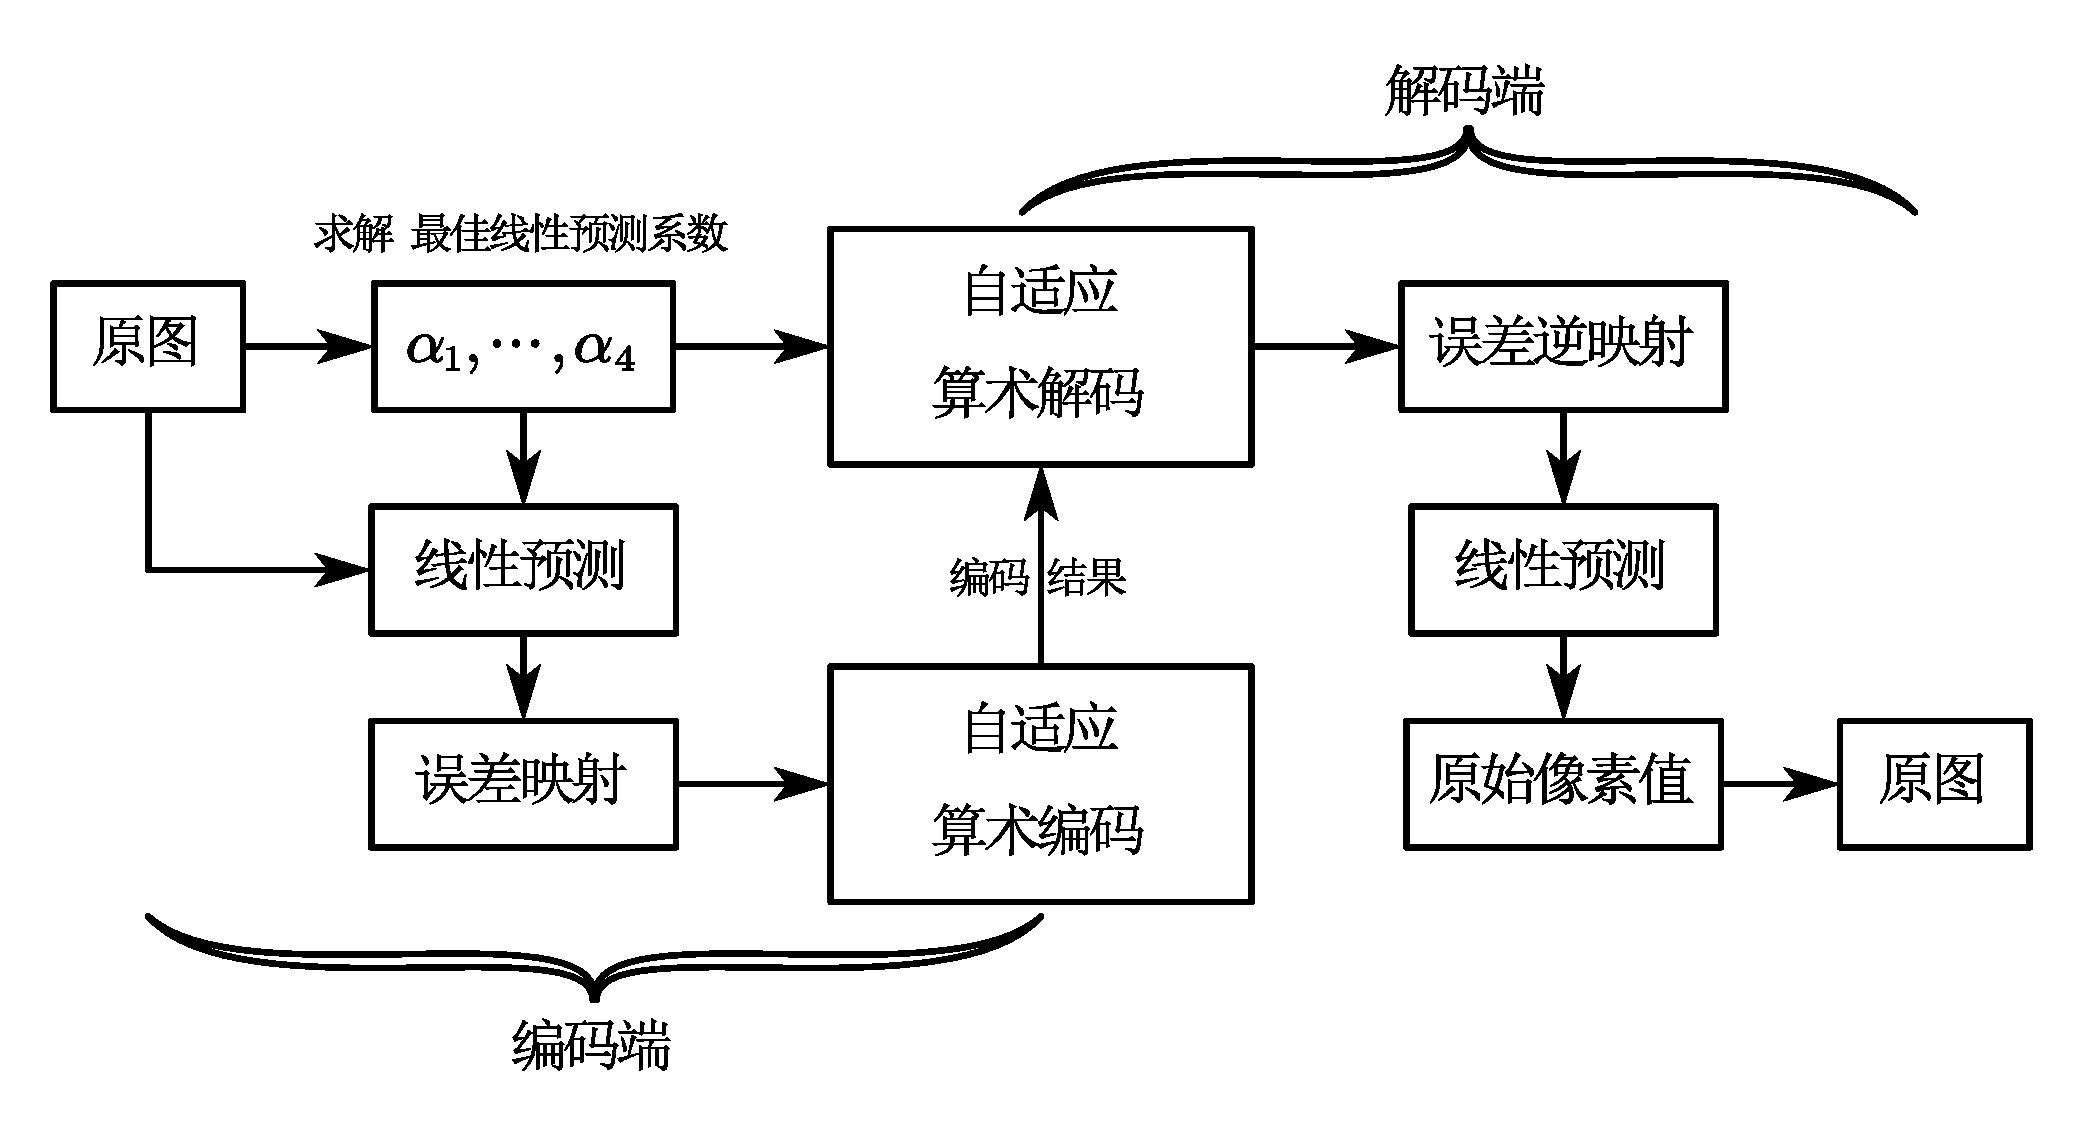
\includegraphics[scale=0.37,trim=0 20 0 20,clip]{imgs/LPC flow.pdf}
    %图片裁剪  trim=左 下 右 上,clip  单位像素
    \caption{线性预测的无失真图像编码方案框架示意图}
    \label{fig: system structure}
\end{figure}

在该编解码系统中:

编码端:对待编码压缩的图像进行遍历,并按最佳线性预测法求解出最佳预测系数;
再对图像进行线性预测和误差映射,减小图像像素值的范围,即使待编码符号以较大的概率分布于零值附近,
继而实现在熵编码中的较短码子表示,提高了编码效率;其中熵编码过程,基于经典的算术编码[1],
对其算法进行改进,采用自适应概率统计法,优化了传统算术编码不适用于长度较大的信源编码问题。

解码端:目的通过编码结果,还原出压缩前的数据信息,作为编码的逆过程,
与编码端工作相似但相逆,此处便不再叙述,需要注意的是,
最佳线性预测解码中,需要将编码端求解的最佳预测系数同编码结果一同传到解码端。


\subsection{线性预测编码}
\subsubsection{线性预测编码原理}
设当前像素为$x_0$,上一像素为$x_1$,则用上一像素作为当前像素的估计得到$x'=x_1$;
预测估计误差为$e=x_0-x'$(像素真值减掉像素估计值得到像素估计误差);

本文利用自然图像的空间相关性,选用邻近四个像素按如下式(\ref{equ: prediction})所示的预测方法:
\begin{equation}
    x'=\alpha_1x_1+\alpha_2x_2+\alpha_3x_3+\alpha_4x_4
    \label{equ: prediction}
\end{equation}

其中:$x_1, x_2, x_3, x_4$与$x_0$均为一幅数字图像中的像素,
且$x_1, x_2, x_3, x_4$从时间因果关系上来说,出现在$x_0$之前,
它们在一幅连续的图像中的位置如下图 \ref{fig: pos of pixel} 所示,$x_0$为边界像素时,取不到的$x_i$值为$0$,
预测估计误差为$e=x_0-x'$。
\begin{figure}[thb] \centering
    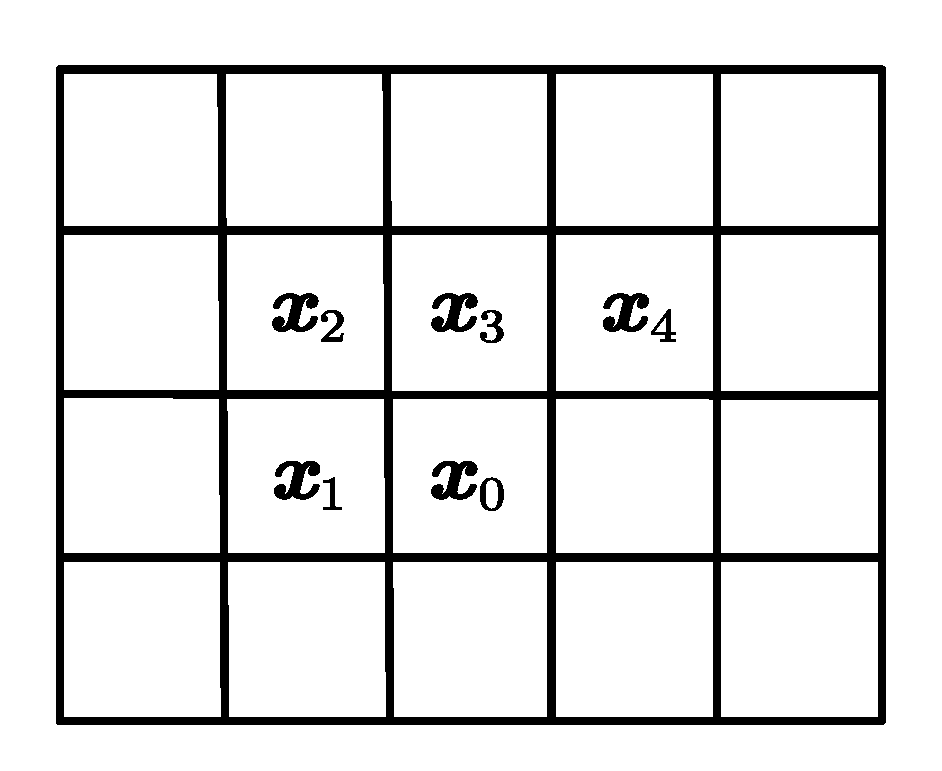
\includegraphics[scale=0.3,trim=0 15 0 20,clip]{imgs/pixel pos.pdf}
    \caption{像素位置示意图}
    \label{fig: pos of pixel}
\end{figure}

若信号是连续变化的,则相邻像素的灰度值将较为相近。利用相邻像素对当前像素作预测后,
预测误差$e$的概率分布将出现误差幅值在$0$附近的概率很大,而误差幅值越大,出现的机会就越小的情况,
这意味着预测误差的熵较小。利用熵编码就能实现对图像的有效压缩。

\subsubsection{利用预测值缩减预测误差取值范围}
由于图像像素$x_0$的灰度取值范围为$0\sim 255$,预测值$x'$取值范围也为$0\sim 255$,
预测误差的取值范围应该是$-255\sim 255$,一共$511$种不同取值,这样每个误差值的平均编码比特数将较多。

但是在考虑到预测值$x'$是已知的情况下,预测误差$e=x_0-x'$的实际取值范围将小得多。
当$e>0$时,它的取值范围只能是$0\sim 255-x'$,而当$e<0$时它的取值范围只能是$-x'\sim 0$。
所以我们可以据此来将预测误差映射到取值范围较小的空间中。设预测误差映射值为$E=E(e)$。

其映射关系如式(\ref{equ: mapping1}, \ref{equ: mapping2})下所示:

如果$0\le x'<128$:
\begin{equation}
    E\left( e \right) =\left\{ \begin{matrix}
        -2e,  & e\le 0      \\
        2e-1, & 0<e\le x'+1 \\
        e+x', & e>x'+1      \\
    \end{matrix} \right.
    \label{equ: mapping1}
\end{equation}

如果$128\le x'<256$:
\begin{equation}
    E\left( e \right) =\left\{ \begin{matrix}
        2e,        & e\ge 0        \\
        -2e-1,     & x'-256\le e<0 \\
        -e+x'-255, & e<x'-256      \\
    \end{matrix} \right.
    \label{equ: mapping2}
\end{equation}

在解码端,逆映射关系如式(\ref{equ: inv mapping1}, \ref{equ: inv mapping2})下所示:

如果$0\le x'<128$:
\begin{equation}
    e=\left\{ \begin{matrix}
        -\frac{E}{2},  & E\le 2x'+1\text{且}E\text{为偶数} \\
        \frac{E+1}{2}, & E\le 2x'+1\text{且}E\text{为奇数} \\
        E-x',          & E>2x'+1                           \\
    \end{matrix} \right.
    \label{equ: inv mapping1}
\end{equation}

如果$128\le x'<256$:
\begin{equation}
    e=\left\{ \begin{matrix}
        \frac{E}{2},    & E\le 511-2x'\text{且}E\text{为偶数} \\
        -\frac{E+1}{2}, & E\le 511-2x'\text{且}E\text{为奇数} \\
        255-x'-E,       & E>511-2x'                           \\
    \end{matrix} \right.
    \label{equ: inv mapping2}
\end{equation}


\subsubsection{最佳线性预测}
若能求出周围像素每一个的最佳权重,即计算出(\ref{equ: prediction})式中各$\alpha_i,(i=1,\cdots,4)$的值,
称为最佳线性预测系数,并求出最佳线性预测值,则可以再次提高压缩效率。

为求解最佳线性预测系数,最佳的目标是让预测误差的平方平均值$E[e^2]$最小,
通过求$E[e^2]$对所有的$\alpha_i$的偏导数为$0$,如下:
\begin{equation}
    \frac{\partial E\left[ e^2 \right]}{\partial \alpha_i}=E\left[
        \frac{\partial}{\partial \alpha_i}\left( x_0-\sum_{k=1}^4{\alpha_k x_k} \right) ^2
        \right] =-2E\left[ ex_i \right] =0
    \label{equ: the best weight}
\end{equation}

得:
\begin{equation}
    -2E\left[ x_ie \right] =-2E\left[ x_i\left( x_0-\sum_{k=1}^4{\alpha_kx_k} \right) \right] =0
    \label{euq: alpha solution1}
\end{equation}

化简:
\begin{equation}
    E\left[ x_i\sum_{k=1}^4{\alpha_kx_k} \right] =E\left[ x_ix_0 \right]
    \label{euq: alpha solution2}
\end{equation}

令$R_{i0}=E\left[ x_ix_0 \right] ,\ R_{ik}=E\left[ x_ix_k \right]$,
即可将(\ref{euq: alpha solution2})式转换为矩阵的形式:
\begin{equation}
    \left[ \begin{matrix}
            R_{11} & R_{12} & R_{13} & R_{14} \\
            R_{21} & R_{22} & R_{23} & R_{24} \\
            R_{31} & R_{32} & R_{33} & R_{34} \\
            R_{41} & R_{42} & R_{43} & R_{44} \\
        \end{matrix} \right] \begin{matrix}
        \left[ \begin{array}{c}
                       \alpha_1 \\
                       \alpha_2 \\
                       \alpha_3 \\
                       \alpha_4 \\
                   \end{array} \right] & =\left[ \begin{array}{c}
                                                     R_{10} \\
                                                     R_{20} \\
                                                     R_{30} \\
                                                     R_{40} \\
                                                 \end{array} \right] \\
    \end{matrix}
    \label{equ: matrix of weight}
\end{equation}

求解方程(\ref{equ: matrix of weight})就可以求出最佳预测系数$\alpha_i$。
再根据最佳预测系数再次对图像进行编码,压缩效率会得到进一步提高。


\subsection{自适应算术编码}
算术编码AC于1979年被提出\cite[]{Rissanen1979ArithmeticCoding},根据概率分布将信源符号映射到$[0,1]$之间,
其编码示意图如下图\ref{fig: arithmetic coding}所示:
\begin{figure}[thb] \centering
    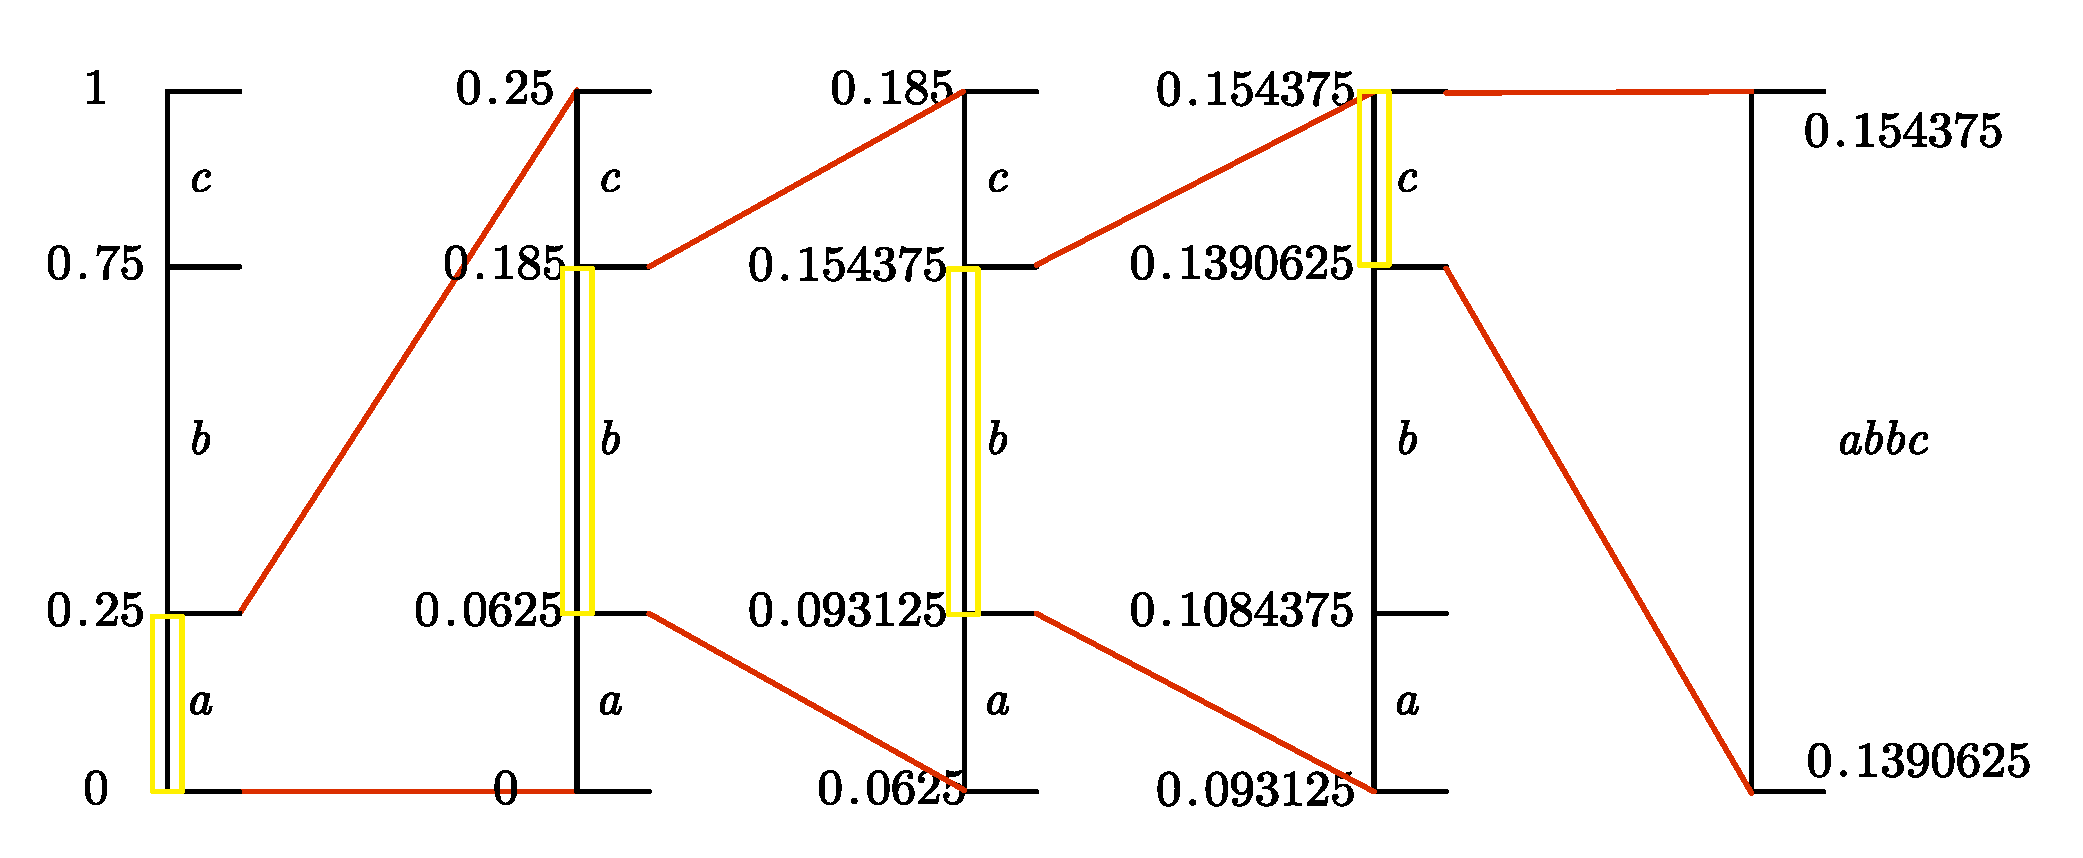
\includegraphics[scale=0.35,trim=0 10 0 10,clip]{imgs/Arithmetic coding.pdf}
    \caption{算术编码原理说明}
    \label{fig: arithmetic coding}
\end{figure}

如图\ref{fig: arithmetic coding}为信源$“abbc”$的算术编码过程,根据各符号的概率分布,以及符号顺序,
计算信源的分配区间,最终使用该区间内的一个数对信源进行表示(图示$“abbc”$可以由$[0.1390625,0.154375]$中的任一小数表示)。

由于AC在编码前,需要遍历信源求解其概率分布,不适用于长信源编码问题中,于是针对任意信源长度的AAC算法被提出
\cite[]{Moffat1990LinearTimeAdaptive},
对于信源$“abbc”$其编码示意图如下图\ref{fig: adaptive arithmetic coding}所示:
\begin{figure}[thb] \centering
    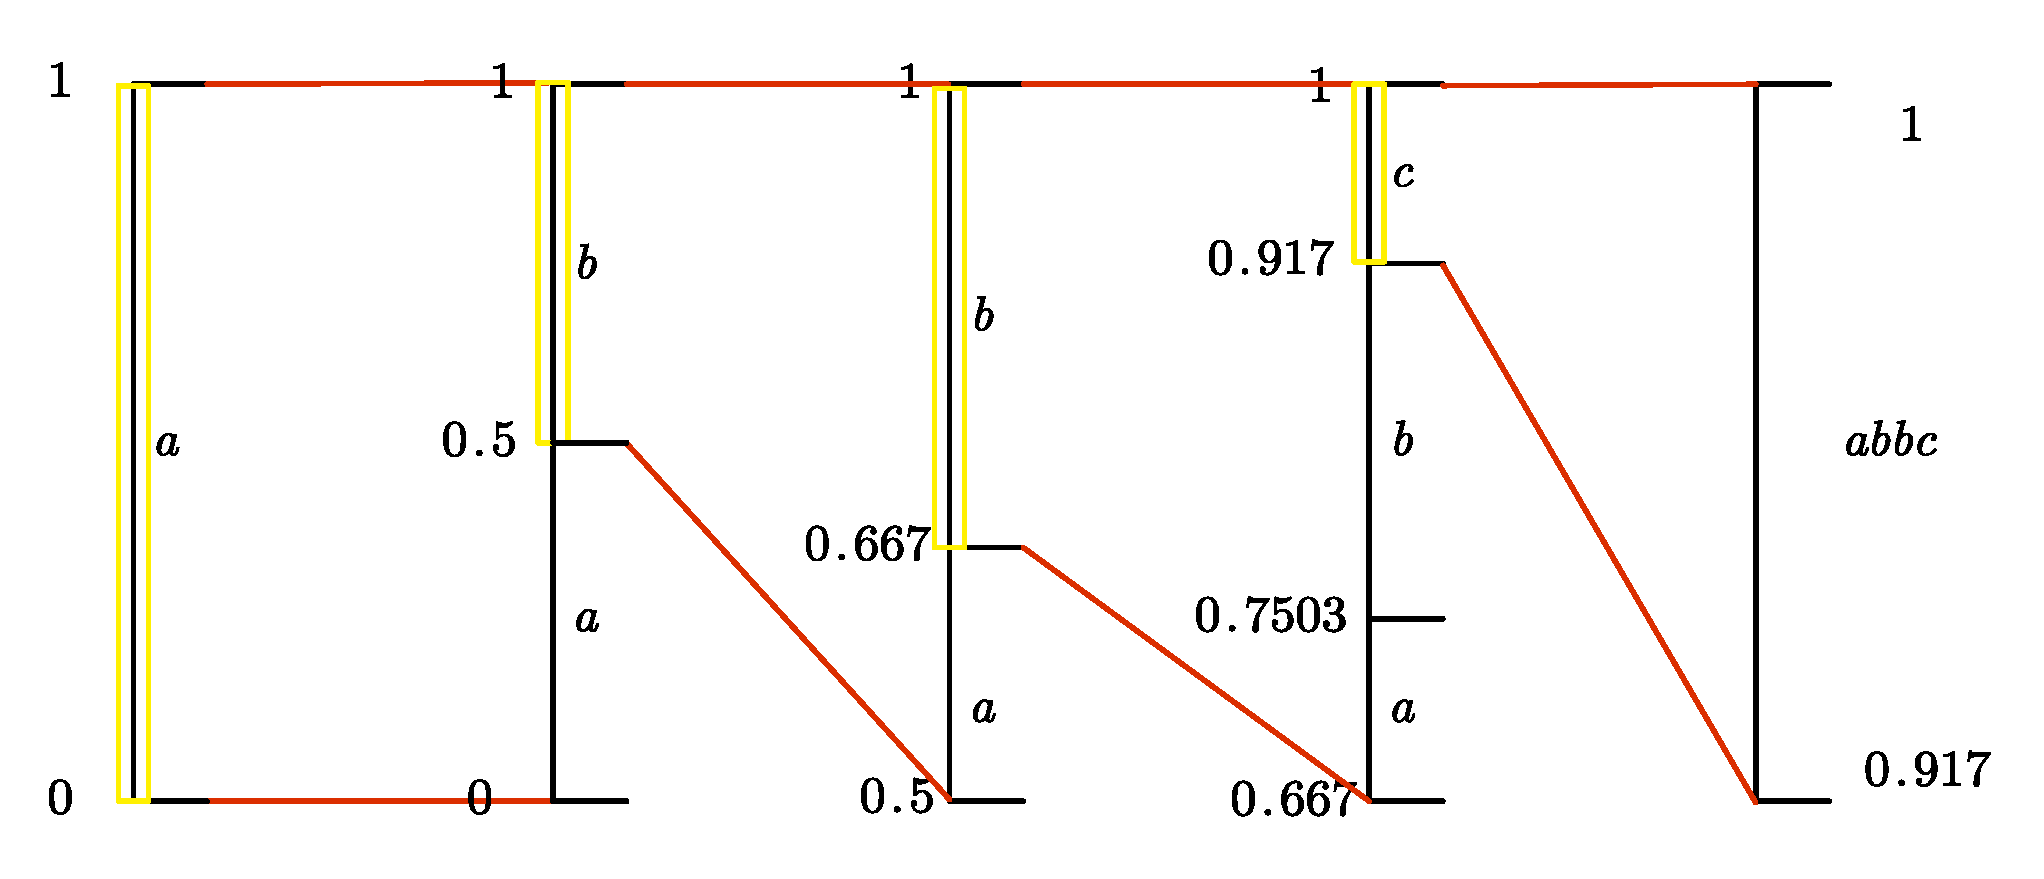
\includegraphics[scale=0.35,trim=0 15 0 30,clip]{imgs/Adaptive arithmetic coding.pdf}
    \caption{算术编码原理说明}
    \label{fig: adaptive arithmetic coding}
\end{figure}

\vspace{-0.2em}
如图\ref{fig: adaptive arithmetic coding}所示,AAC在编码前无需一直信源符号的概率分布,且无关信源长度,
其区间分布取决于以编码信源的长度,相对AC降低了时间复杂度,且推广了适用范围。


\section{实验}
本文测试实验图像(均为$512\times 512, .raw$格式)如下图\ref{fig: img set}所示:
\vspace{-0.2em}
\begin{figure}[thb] \centering
    \subfigure[airplane]{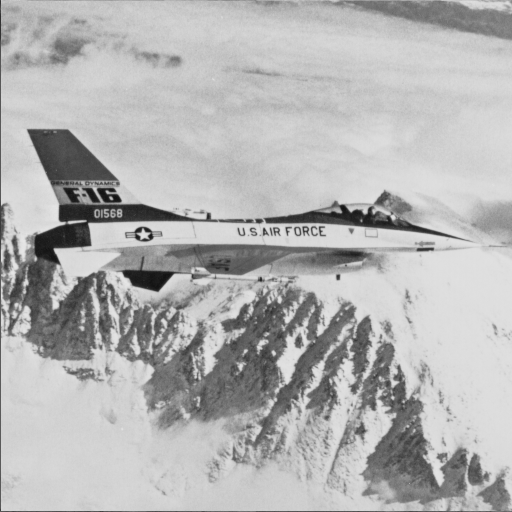
\includegraphics[width=2.5cm]{imgs/airplane.png}}
    \subfigure[baboon]{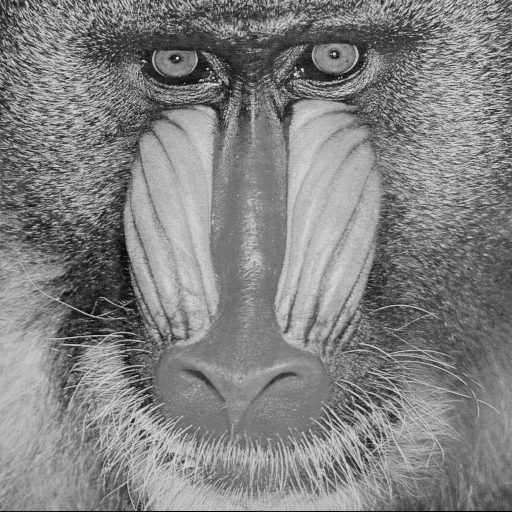
\includegraphics[width=2.5cm]{imgs/baboon.png}}
    \subfigure[cameraman]{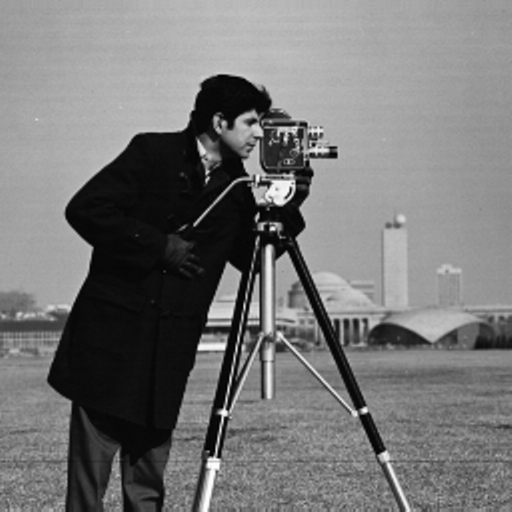
\includegraphics[width=2.5cm]{imgs/cameraman.png}}
    \subfigure[lena]{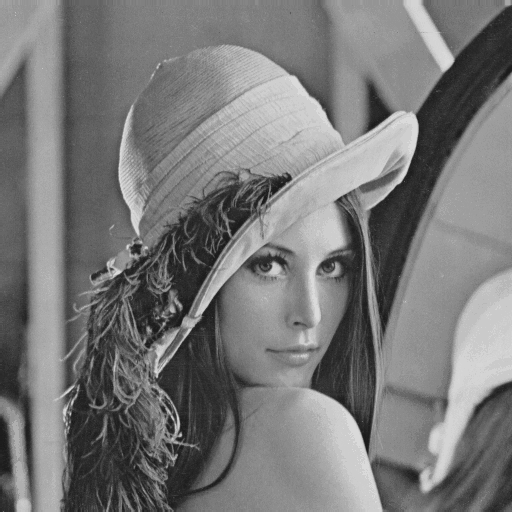
\includegraphics[width=2.5cm]{imgs/lena.png}}
    \subfigure[woman]{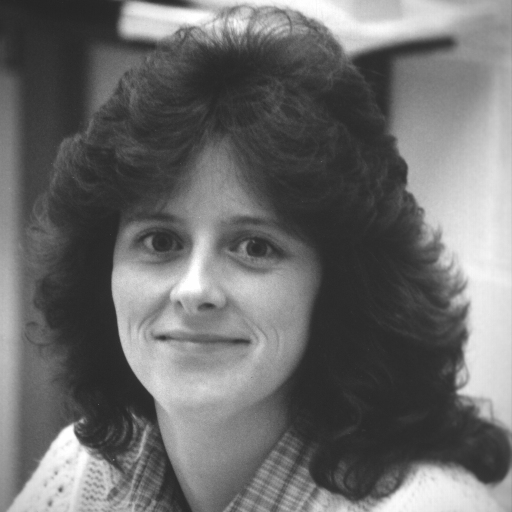
\includegraphics[width=2.5cm]{imgs/woman_darkhair.png}}
    \vspace{-0.2em}
    \caption{实验测试图像集}
    \label{fig: img set}
\end{figure}

\vspace{-0.3em}
首先对待编码图像求解最佳线性预测系数$\alpha_1 \sim \alpha_4$(保留四位小数),如下表\ref{tab: the best weight}所示:
\begin{table}[htbp]
    \centering
    \vspace{-0.3em}
    \caption{最佳系数求解结果}
    \vspace{-0.4em}
    \begin{tabular}{c|ccccc}
        \toprule
                   & airplane & baboon  & cameraman & lena    & woman   \\
        \midrule
        $\alpha_1$ & 0.8882   & 0.6975  & 0.9224    & 0.7263  & 0.8896  \\
        $\alpha_2$ & -0.7260  & -0.1245 & -0.8550   & -0.5222 & -0.8059 \\
        $\alpha_3$ & 0.8083   & 0.3047  & 0.9114    & 0.6616  & 0.8924  \\
        $\alpha_4$ & 0.0296   & 0.119   & 0.0209    & 0.1345  & 0.0243  \\
        \bottomrule
    \end{tabular}%
    \label{tab: the best weight}
\end{table}%

其中$\alpha_1$和$\alpha_3$比较大,$\alpha_2$为负值,说明在连续图像中,像素值与其左侧和上侧像素值最接近,
与左上和右上相似较远。

各图像压缩率,如下表\ref{tab: compression rate}所示:
\begin{table}[htbp]
    \centering
    \caption{图像压缩率结果}
    \begin{tabular}{c|ccc}
        \toprule
        \multirow{2}[4]{*}{\textbf{图像}} & \multicolumn{3}{c}{\textbf{压缩方式}}                                                         \\
        \cmidrule{2-4}                    & \multicolumn{1}{c|}{\textbf{经典LPC}} & \multicolumn{1}{c|}{\textbf{最佳LPC}} & \textbf{提升} \\
        \midrule
        airplane                          & 43.08\%                               & 46.42\%                               & 3.34\%        \\
        baboon                            & 19.74\%                               & 22.55\%                               & 2.81\%        \\
        cameraman                         & 48.26\%                               & 57.08\%                               & 8.82\%        \\
        lena                              & 41.93\%                               & 43.16\%                               & 1.23\%        \\
        woman                             & 51.96\%                               & 52.73\%                               & 0.76\%        \\
        \bottomrule
    \end{tabular}%
    \label{tab: compression rate}
\end{table}%

由上表\ref{tab: compression rate}可知,使用最佳LPC对图像的无损压缩率能够接近$50\%$,
对于baboon此类高频信息更多的图像压缩率会降低,在cameraman此类更为平滑的图像中压缩率最高,
说明LPC无损压缩更适用于平滑,含整块相似的图像中。
通过对比经典LPC算法和最佳LPC算法,发现压缩率平均提升了$3.5\%$,
且在cameraman此类平滑图像中,最佳LPC相较于经典LPC算法,压缩效率提升更为明显,达到了$8.82\%$的提升。


\section{结论}
本文提出了一种基于线性预测的图像无失真编码方案,求解最佳系数进行线性预测,
并通过分析误差取值范围,使得预测误差以更大的概率映射到零值附近,
降低了描述信源所需的信息度量;并对映射后的误差,进行自适应算术编码,
在不增加算法复杂度的同时,提高了编码效率。

实验得出,使用最佳LPC编码对图像的无损压缩率接近$50\%$,
同在无失真前提下,最佳LPC编码,相较于传统LPC方案,压缩效率平均提高了$3.5\%$,
且在平滑图像中,最佳LPC相较于经典LPC算法,压缩效率提升更为明显,在cameraman测试图像中,压缩率达到了$8.82\%$的提升。


% 指定.bib文件,插入参考文献,不加文件后缀
\bibliography{ref}
% 参考文献格式
\bibliographystyle{IEEEtran}

\clearpage
\appendix
\section{附录概览}
本文实验的程序及论文排版 \LaTeX 代码见github:
\href{https://github.com/nayuki/Reference-arithmetic-coding/tree/master/java}{A Lossless Image Coding Based on LPC}
,其中的自适应算术编码基于工程:
\href{https://github.com/nayuki/Reference-arithmetic-coding/tree/master/java}
{https://github.com/nayuki/Reference-arithmetic-coding/tree/master/java}。

其他附录如下:
\begin{description}
    \item[Matlab 最佳系数求解:] 为最佳线性预测系数求解程序,使用MATLAB实现;
    \item[Java Main 程序:] 编解码调用主程序,使用Java实现;
    \item[Java LPC-AAC 编码:] 基于线性预测的自适应算术编码程序,使用Java实现;
    \item[Java LPC-AAC 解码:] 基于线性预测的自适应算术解码程序,使用Java实现。
\end{description}

\section{实验程序}
\lstinputlisting[language=Matlab, caption={Matlab 最佳系数求解程序}]{codes/Best_weight_LPC.m}
\lstinputlisting[language=Java, caption={Java Main 程序}]{codes/main_LPC.java}
\lstinputlisting[language=Java, caption={Java LPC-AAC 编码程序}]{codes/LPC_compress.java}
\lstinputlisting[language=Java, caption={Java LPC-AAC 解码程序}]{codes/LPC_decompress.java}


\end{document}
